\scanpage{142}
{\ttfamily
TRACEUR J\quad BUFFER 1020\quad BANDE 9 PISTES\quad PLUMES : 3\quad XMAX = 10100.0\quad YMAX = 70.0\quad STNB = 100.00000\\
25/ 8/ 82\qquad 10 HEURES 57 MINUTES\\
JOB\qquad BANDE IBM NUMERO\\
\hspace*{3em}****************************************\\
TRACEUR UTILISE\\
REMISE DE LA BANDE\\
DEBUT DE TRAITEMENT\\
FIN DE TRAITEMENT\\
REMISE DES GRAPH.\\
INCIDENTS SURVENUS
\[
\begin{array}{lllll}
\texttt{PLOT 4B}&\texttt{\unsure{BLANC|ELANC}}&&0&0\\
\texttt{CNU*0202 GRAPHI1}&\texttt{JB 82237 105600}&&0&0\\
\texttt{GRAPHI1 CNU*0202 82237 M06 P02900500}&7&0&0&0\quad4
\end{array}
\]
}
\figure{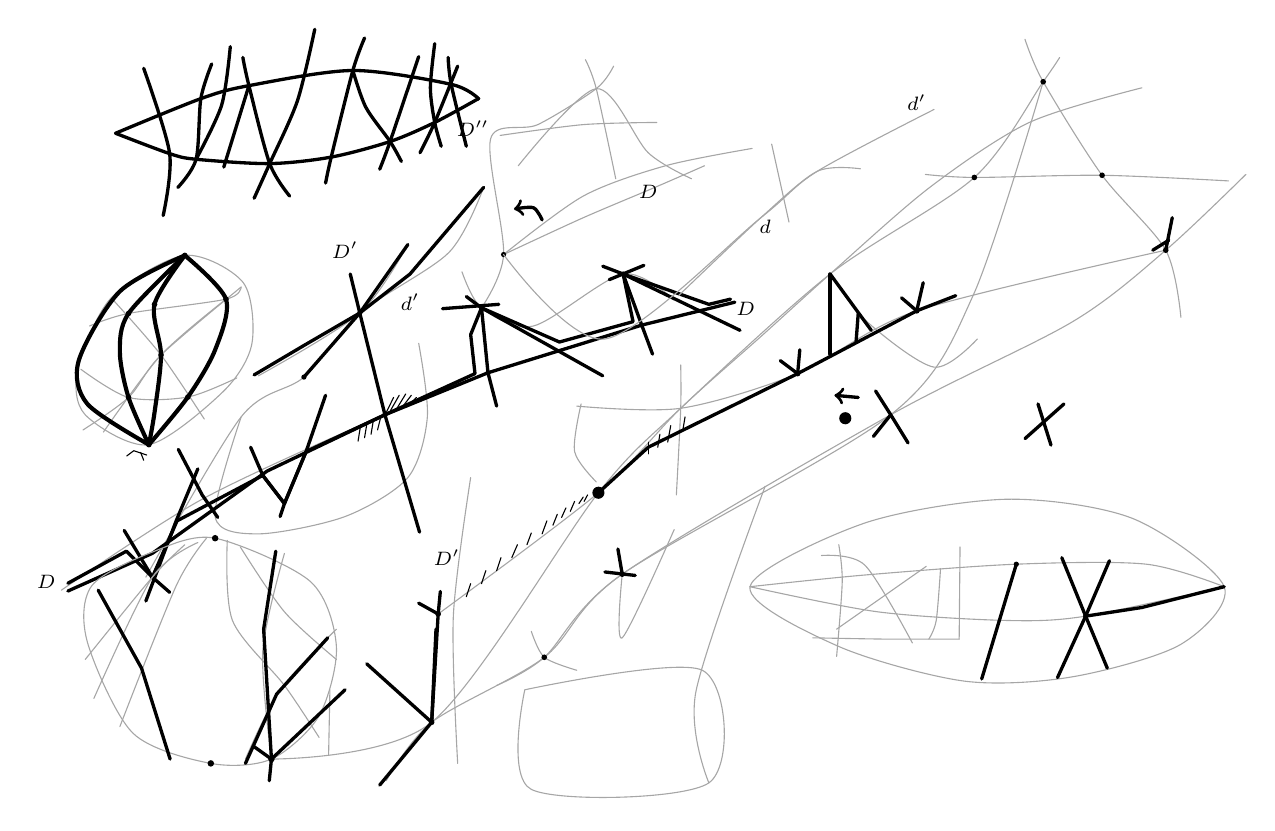
\begin{tikzpicture}[x=.55cm,y=-.55cm,line cap=round,line join=round,g/.style={olive!80!yellow,line width=1.7pt},r/.style={orange!80!brown,line width=1.8pt},w/.style={red!60!black,line width=1.5pt},b/.style={blue!60!black,line width=1.4pt},p/.style={gray!70,thin},k/.style={black,line width=1.2pt},every node/.style={font=\scriptsize}]
% Upper-left lens and crossing strands.
\draw[k] plot[smooth] coordinates {(2.7,4.75) (4.67,3.95) (5.78,3.65) (8.18,3.3) (10.45,3.62) (11.08,3.95)};
\draw[k] plot[smooth] coordinates {(2.7,4.75) (3.95,5.22) (4.56,5.35) (6.26,5.45) (7.68,5.3) (9.04,4.94) (10.07,4.5) (11.08,3.95)};
\draw[k] plot[smooth] coordinates {(3.35,3.25) (3.95,5.22) (3.8,6.65)};
\draw[k] plot[smooth] coordinates {(4.92,3.15) (4.67,3.95) (4.56,5.35) (4.14,6.0)};
\draw[k] plot[smooth] coordinates {(5.35,2.75) (5.15,4.1) (4.56,5.35)};
\draw[k] plot[smooth] coordinates {(5.78,3.65) (5.2,5.53)};
\draw[k] plot[smooth] coordinates {(5.64,3.0) (5.78,3.65) (6.26,5.45) (6.72,6.2)};
\draw[k] plot[smooth] coordinates {(7.3,2.35) (6.9,4.0) (6.26,5.45) (5.9,6.25)};
\draw[k] plot[smooth] coordinates {(8.45,2.55) (8.18,3.3) (7.68,5.3) (7.55,5.9)};
\draw[k] plot[smooth] coordinates {(8.18,3.3) (8.48,4.15) (9.04,4.94) (9.3,5.4)};
\draw[k] plot[smooth] coordinates {(9.7,2.98) (9.04,4.94) (8.8,5.58)};
\draw[k] plot[smooth] coordinates {(10.07,2.68) (9.97,3.7) (10.07,4.5) (10.22,5.05)};
\draw[k] plot[smooth] coordinates {(10.38,3.0) (10.45,3.62) (10.8,5.05)};
\draw[k] plot[smooth] coordinates {(10.6,3.2) (10.07,4.5) (9.73,5.2)};
\fill[k] (3.95,5.22) circle (.045);
\fill[k] (4.67,3.95) circle (.045);
\fill[k] (4.56,5.35) circle (.045);
\fill[k] (5.78,3.65) circle (.045);
\fill[k] (6.26,5.45) circle (.045);
\fill[k] (8.18,3.3) circle (.045);
\fill[k] (7.68,5.3) circle (.045);
\fill[k] (9.04,4.94) circle (.045);
\fill[k] (10.07,4.5) circle (.045);
\fill[k] (10.45,3.62) circle (.045);
\fill[k] (11.08,3.95) circle (.045);
\node at (10.95,4.65) {$D^{\prime\prime}$};
% Left middle globe, with pencil arcs behind ink arcs.
\draw[p] plot[smooth cycle] coordinates {(4.3,7.57) (5.65,8.2) (5.85,9.6) (5.2,10.7) (3.47,11.94) (2.0,11.25) (1.83,10.2) (2.6,8.55)};
\draw[p] plot[smooth] coordinates {(1.9,10.2) (3.0,10.85) (4.37,10.84) (5.5,10.4)};
\draw[p] plot[smooth] coordinates {(2.1,9.2) (3.0,8.91) (5.25,8.58) (5.6,8.3)};
\draw[p] plot[smooth] coordinates {(2.42,11.65) (3.75,9.87) (5.25,8.58)};
\draw[p] plot[smooth] coordinates {(2.6,8.55) (3.75,9.87) (4.75,11.35)};
\draw[p] plot[smooth] coordinates {(1.95,11.6) (3.0,10.85) (3.75,9.87) (5.6,8.3)};
\draw[k,line width=1.5pt] plot[smooth] coordinates {(4.3,7.57) (2.8,8.4) (1.85,10.0) (2.05,11.0) (3.47,11.94)};
\draw[k,line width=1.5pt] plot[smooth] coordinates {(4.3,7.57) (5.25,8.58) (5.0,9.75) (4.37,10.84) (3.47,11.94)};
\draw[k,line width=1.5pt] plot[smooth] coordinates {(4.3,7.57) (3.0,8.91) (2.8,9.8) (3.0,10.85) (3.47,11.94)};
\draw[k,line width=1.5pt] plot[smooth] coordinates {(4.3,7.57) (3.6,8.7) (3.75,9.87) (3.6,11.2) (3.47,11.94)};
\fill[k] (4.3,7.57) circle (.065);
\fill[k] (3.0,8.91) circle (.065);
\fill[k] (3.6,8.7) circle (.065);
\fill[k] (5.25,8.58) circle (.065);
\fill[k] (3.75,9.87) circle (.065);
\fill[k] (3.0,10.85) circle (.065);
\fill[k] (4.37,10.84) circle (.065);
\fill[k] (3.47,11.94) circle (.065);
\draw[k,thin] (2.96,12.2)--(3.12,12.08)--(3.42,12.18);
\draw[k,thin] (3.28,12.12)--(3.35,12.3);
% Central oblique line D and its black/pencil crossing sketches.
\draw[p] plot[smooth] coordinates {(1.45,15.3) (4.7,13.2) (8.9,11.25) (11.3,10.28) (14.85,9.18) (17.0,8.65)};
\draw[p] plot[smooth] coordinates {(3.4,15.0) (5.6,11.3) (7.05,10.38) (8.34,8.9) (10.4,7.5) (11.2,6.0)};
\draw[p] plot[smooth] coordinates {(6.0,10.35) (8.34,8.9) (9.45,7.32)};
\draw[p] plot[smooth] coordinates {(8.34,8.9) (8.92,11.25) (9.72,13.96)};
\draw[p] plot[smooth] coordinates {(5.6,11.3) (5.0,13.6) (6.0,14.0) (8.0,13.6) (9.45,12.7) (9.9,11.3) (9.7,9.6)};
\draw[p] plot[smooth] coordinates {(10.7,7.95) (11.15,8.78) (12.35,9.2) (14.42,8.0) (15.6,8.6)};
\draw[p] plot[smooth] coordinates {(11.15,8.78) (11.66,7.55) (11.36,4.88) (12.45,4.55) (13.8,3.72) (14.2,3.2)};
\draw[p] plot[smooth] coordinates {(11.66,7.55) (13.5,6.7) (15.2,5.98) (16.3,5.5)};
\draw[p] plot[smooth] coordinates {(12.0,5.5) (13.8,3.72) (15.0,5.2) (16.0,5.8)};
\draw[p] plot[smooth] coordinates {(13.55,3.05) (13.8,3.72) (14.25,5.8)};
\draw[p] plot[smooth] coordinates {(11.58,4.8) (13.5,4.55) (15.2,4.5)};
\draw[p] plot[smooth] coordinates {(11.66,7.55) (13.5,6.2) (15.4,5.5) (17.4,5.1)};
\draw[k] (1.6,15.14)--(2.95,14.4)--(3.55,15.0)--(4.12,13.7)--(6.1,12.65)--(6.6,13.3)--(7.1,12.1)--(8.92,11.25)--(11.0,10.3)--(10.9,9.4)--(11.15,8.78)--(12.95,9.57)--(14.65,9.1)--(14.42,8.0)--(16.4,8.7)--(16.9,8.58);
\draw[k] (1.6,15.32)--(3.55,14.45)--(6.2,12.55)--(8.92,11.25)--(11.3,10.28)--(14.85,9.18)--(17.0,8.65);
\draw[k] (3.4,15.55)--(4.1,13.7)--(4.6,12.5);
\draw[k] (2.9,13.92)--(3.55,15.0)--(3.95,15.35);
\draw[k] (4.15,12.05)--(4.7,13.1)--(5.06,13.62);
\draw[k] (5.82,12.0)--(6.1,12.65)--(6.6,13.3)--(6.5,13.6);
\draw[k] (7.55,10.8)--(7.1,12.1)--(6.6,13.3);
\draw[k] (5.9,10.33)--(7.05,9.65)--(8.34,8.9)--(9.45,7.32);
\draw[k] (7.05,10.38)--(8.34,8.9)--(9.5,8.0)--(11.2,6.0);
\draw[k] (8.12,8.0)--(8.34,8.9)--(8.92,11.25)--(9.72,13.96);
\draw[k] (10.8,8.52)--(11.15,8.78)--(13.95,10.35);
\draw[k] (11.15,8.78)--(11.3,10.28)--(11.5,11.05);
\draw[k] (10.25,8.8)--(11.55,8.7);
\draw[k] (13.95,7.82)--(14.42,8.0)--(17.12,9.3);
\draw[k] (14.42,8.0)--(14.85,9.18)--(15.1,9.85);
\draw[k] (14.1,8.13)--(14.9,7.8);
\draw[k,thin] (8.3,11.86)--(8.35,11.55);
\draw[k,thin] (8.45,11.78)--(8.5,11.48);
\draw[k,thin] (8.6,11.7)--(8.65,11.4);
\draw[k,thin] (8.75,11.6)--(8.82,11.32);
\draw[k,thin] (8.95,11.2)--(9.12,10.85);
\draw[k,thin] (9.05,11.15)--(9.25,10.8);
\draw[k,thin] (9.18,11.13)--(9.4,10.77);
\draw[k,thin] (9.3,11.1)--(9.53,10.8);
\draw[k,thin] (9.42,11.07)--(9.65,10.85);
\fill[k] (3.55,15.0) circle (.06);
\fill[k] (7.05,10.38) circle (.06);
\fill[k] (8.34,8.9) circle (.06);
\fill[k] (8.92,11.25) circle (.06);
\fill[k] (11.15,8.78) circle (.06);
\fill[k] (11.3,10.28) circle (.06);
\fill[k] (14.42,8.0) circle (.06);
\fill[k] (14.85,9.18) circle (.06);
\fill[k] (11.66,7.55) circle (.06);
\node at (1.1,15.12) {$D$};
\node at (8.0,7.45) {$D^{\prime}$};
\node at (9.5,8.65) {$\unsure{d^{\prime}}$};
\node at (15.0,6.1) {$D$};
\node at (17.25,8.8) {$D$};
\node at (10.35,14.55) {$\unsure{D^{\prime}}$};
\draw[k,->] plot[smooth] coordinates {(12.55,6.75) (12.35,6.47) (11.9,6.5)};
% Upper-right and central-right pencil arrangement and darker local pieces.
\draw[p] plot[smooth] coordinates {(10.15,15.85) (13.85,13.05) (15.75,11.1) (17.65,9.4) (19.2,8.0) (21.5,6.0) (23.8,4.5) (26.4,3.7)};
\draw[p] plot[smooth] coordinates {(6.3,19.2) (10.0,18.35) (13.85,13.05) (15.75,11.1) (19.2,8.0) (22.53,5.77) (24.12,3.56) (24.5,3.0)};
\draw[p] plot[smooth] coordinates {(8.95,19.7) (10.0,18.35) (12.6,16.85) (14.4,14.93) (20.6,11.25) (24.8,9.1) (26.95,7.45) (28.8,5.7)};
\draw[p] plot[smooth] coordinates {(11.5,17.5) (12.6,16.85) (14.4,14.93) (20.6,11.25) (22.5,8.5) (24.12,3.56)};
\draw[p] plot[smooth] coordinates {(11.66,7.55) (14.0,9.5) (17.6,6.7) (18.9,5.63) (21.6,4.2)};
\draw[p] plot[smooth] coordinates {(15.7,8.5) (17.6,6.7) (18.9,5.63) (19.9,5.57)};
\draw[p] plot[smooth] coordinates {(17.85,5.0) (18.25,6.8)};
\draw[p] plot[smooth] coordinates {(13.35,11.05) (15.75,11.1) (18.45,10.3) (21.2,8.85) (26.95,7.45)};
\draw[p] plot[smooth] coordinates {(21.4,5.7) (22.53,5.77) (25.48,5.72) (28.4,5.85)};
\draw[p] plot[smooth] coordinates {(23.7,2.58) (24.12,3.56) (25.48,5.72) (26.95,7.45) (27.3,9.0)};
\draw[p] plot[smooth] coordinates {(19.2,8.0) (20.05,9.1) (21.6,10.15) (22.6,9.5)};
\draw[p] plot[smooth] coordinates {(13.8,12.8) (13.3,12.1) (13.45,11.0)};
\draw[p] plot[smooth] coordinates {(15.75,10.1) (15.75,11.1) (15.65,13.1)};
\draw[p] plot[smooth] coordinates {(14.4,14.93) (14.4,16.4) (15.6,13.9)};
\draw[p] plot[smooth] coordinates {(12.3,16.25) (12.6,16.85) (13.35,17.15)};
\draw[p] plot[smooth] coordinates {(17.7,12.9) (16.1,17.65) (16.4,19.75)};
\draw[p] plot[smooth] coordinates {(10.9,12.7) (10.5,15.9) (10.6,19.3)};
\draw[p] plot[smooth] coordinates {(12.15,17.6) (16.25,17.15) (16.4,19.75) (12.3,19.9) (12.15,17.6)};
\draw[k] (13.85,13.05)--(15.0,12.0)--(18.45,10.3)--(21.2,8.85);
\draw[k] (10.15,15.85)--(10.0,18.35)--(8.8,19.8);
\draw[k] (18.45,10.3)--(18.05,10.0);
\draw[k] (18.45,10.3)--(18.5,9.75);
\draw[k] (21.2,8.85)--(20.85,8.55);
\draw[k] (21.2,8.85)--(21.35,8.2);
\draw[k] (21.2,8.85)--(22.1,8.5);
\draw[k] (19.2,8.0)--(19.2,9.85);
\draw[k] (19.2,8.0)--(20.15,9.3);
\draw[k] (19.85,8.9)--(19.8,9.56);
\draw[k] (26.95,7.45)--(27.1,6.7);
\draw[k] (26.65,7.45)--(27.02,7.22);
\draw[k] (24.0,11.0)--(24.3,11.95);
\draw[k] (23.7,11.8)--(24.6,11.0);
\draw[k] (14.4,14.93)--(14.3,14.35);
\draw[k] (14.0,14.88)--(14.7,14.96);
\draw[k] (10.15,15.85)--(9.7,15.6);
\draw[k] (10.15,15.85)--(10.2,15.33);
\draw[k] (8.5,17.0)--(10.0,18.35)--(10.1,16.2);
\draw[k] (20.6,11.25)--(20.25,10.7);
\draw[k] (20.6,11.25)--(21.0,11.9);
\draw[k] (20.6,11.25)--(20.2,11.75);
\fill[k] (24.12,3.56) circle (.065);
\fill[k] (22.53,5.77) circle (.065);
\fill[k] (25.48,5.72) circle (.065);
\fill[k] (26.95,7.45) circle (.065);
\fill[k] (18.45,10.3) circle (.065);
\fill[k] (21.2,8.85) circle (.065);
\fill[k] (10.15,15.85) circle (.065);
\fill[k] (10.0,18.35) circle (.065);
\fill[k] (12.6,16.85) circle (.065);
\fill[k] (14.4,14.93) circle (.065);
\fill[k] (13.85,13.05) circle (.14);
\fill[k] (19.55,11.33) circle (.14);
\draw[k,thin] (10.8,15.45)--(10.9,15.15);
\draw[k,thin] (11.15,15.15)--(11.25,14.85);
\draw[k,thin] (11.5,14.85)--(11.6,14.55);
\draw[k,thin] (11.85,14.55)--(11.98,14.25);
\draw[k,thin] (12.2,14.25)--(12.3,13.98);
\draw[k,thin] (12.55,14.0)--(12.66,13.7);
\draw[k,thin] (12.8,13.8)--(12.9,13.55);
\draw[k,thin] (13.0,13.62)--(13.1,13.4);
\draw[k,thin] (13.2,13.48)--(13.3,13.25);
\draw[k,thin] (13.4,13.3)--(13.5,13.15);
\draw[k,thin] (13.52,13.25)--(13.6,13.1);
\draw[k,thin] (15.0,12.15)--(15.0,11.88);
\draw[k,thin] (15.22,12.0)--(15.27,11.7);
\draw[k,thin] (15.45,11.88)--(15.52,11.5);
\draw[k,thin] (15.8,11.6)--(15.85,11.3);
\node at (21.2,4.05) {$d^{\prime}$};
\node at (17.7,6.9) {$d$};
\draw[k,->] plot[smooth] coordinates {(19.85,10.85) (19.3,10.8)};
% Lower-left circle with crossing arcs.
\draw[p] plot[smooth cycle] coordinates {(5.0,14.1) (7.2,15.1) (7.8,16.6) (7.4,18.2) (6.3,19.2) (4.9,19.3) (3.1,18.6) (2.05,16.5) (2.15,15.2) (3.6,14.4)};
\draw[p] plot[smooth] coordinates {(2.2,17.8) (3.55,15.0) (4.6,14.2)};
\draw[p] plot[smooth] coordinates {(2.8,18.45) (4.1,15.2) (4.8,14.1)};
\draw[p] plot[smooth] coordinates {(2.0,16.9) (3.55,15.0) (4.3,14.25)};
\draw[p] plot[smooth] coordinates {(5.28,14.15) (5.4,16.0) (6.6,17.5) (7.4,18.7)};
\draw[p] plot[smooth] coordinates {(5.58,14.3) (6.6,15.8) (7.8,16.9)};
\draw[p] plot[smooth] coordinates {(7.8,16.2) (6.5,17.6) (5.7,19.2)};
\draw[p] plot[smooth] coordinates {(7.65,17.6) (7.62,19.1)};
\draw[p] plot[smooth] coordinates {(6.6,14.45) (6.1,16.7) (6.3,19.2)};
\draw[k] (2.3,15.3)--(3.3,17.1)--(3.96,19.2);
\draw[k] (6.4,14.4)--(6.12,16.2)--(6.3,19.2);
\draw[k] (7.6,16.4)--(6.42,17.7)--(5.7,19.3);
\draw[k] (6.3,19.2)--(8.0,17.6);
\draw[k] (5.88,18.9)--(6.3,19.2)--(6.25,19.7);
\fill[k] (5.0,14.1) circle (.075);
\fill[k] (4.9,19.3) circle (.075);
\fill[k] (6.3,19.2) circle (.075);
% Lower-right elongated lens, with two dark marked crossings.
\draw[p] plot[smooth cycle] coordinates {(17.35,15.22) (20.0,13.75) (23.3,13.2) (26.2,13.65) (28.3,15.22) (27.3,16.55) (24.8,17.3) (22.3,17.4) (19.4,16.6)};
\draw[p] plot[smooth] coordinates {(17.35,15.22) (20.0,14.95) (23.5,14.7) (26.5,14.7) (28.3,15.22)};
\draw[p] plot[smooth] coordinates {(17.35,15.22) (20.3,15.8) (23.3,16.0) (25.1,15.9) (28.3,15.22)};
\draw[p] plot[smooth] coordinates {(19.4,14.25) (19.48,15.1) (19.35,16.83)};
\draw[p] plot[smooth] coordinates {(19.0,14.5) (20.0,14.72) (21.1,16.52)};
\draw[p] plot[smooth] coordinates {(19.35,16.2) (21.42,14.75)};
\draw[p] plot[smooth] coordinates {(22.2,14.3) (22.18,16.43)};
\draw[p] plot[smooth] coordinates {(21.75,14.8) (21.65,16.0) (21.48,16.43)};
\draw[p] plot[smooth] coordinates {(18.8,16.4) (20.5,16.43) (22.18,16.43)};
\draw[k] (22.7,17.35)--(23.5,14.7);
\draw[k] (24.55,14.55)--(25.1,15.9)--(25.6,17.1);
\draw[k] (25.65,14.62)--(25.1,15.9)--(24.45,17.32);
\draw[k] (25.1,15.9)--(26.4,15.7)--(28.3,15.22);
\fill[k] (23.5,14.7) circle (.06);
\fill[k] (25.1,15.9) circle (.06);
\end{tikzpicture}}

$p.r.$ \unsure{stble|stable}\\
$p.r.$ \unsure{semi-stbles|semi-stables}\\
$p.r.$ \uline{critiques} (\unsure{on réserve pour}\\
\unsure{la spécialisation})

\[n\frac{(n-1)(n-2)}{2}\]
\[
\frac12\frac{n(n-1)}2\left(\frac{n(n-1)}2-1\right)
-\frac{n(n-1)(\unsure{n-1|n-2})}{2}
=\quad\deleted{\unsure{n+2}}\quad\sim\frac18n^4
\]
\margin{\mspage{141}}
